% ------------------------------------------------------------------------------
% 6.3. ANÁLISIS DE PAQUETES
% ------------------------------------------------------------------------------
\wfa{\wn{6}.3. Análisis de Paquetes}\label{sec:cap6_analisis_paquetes}

El análisis de paquetes describe cómo se relacionan entre sí los seis paquetes identificados. Una dependencia entre dos paquetes existe cuando un caso de uso de uno de ellos incluye o extiende a un caso de uso del otro, o requiere sus datos para completarse; por ejemplo, el envío de la postulación del paquete Convocatoria y Postulación incluye la precalificación del paquete Preselección con IA. Conocer estas dependencias permite ordenar la construcción del sistema, reducir el acoplamiento y delimitar el alcance de cada iteración.

La Figura~\ref{fig:analisis_paquetes} presenta el diagrama de análisis de paquetes del sistema y las dependencias entre los seis paquetes identificados.

\begin{figure}[H]
\caption{Diagrama de análisis de paquetes del Sistema Web y Móvil de Postulación y Preselección de la Beca Comedor}
\label{fig:analisis_paquetes}
\centering
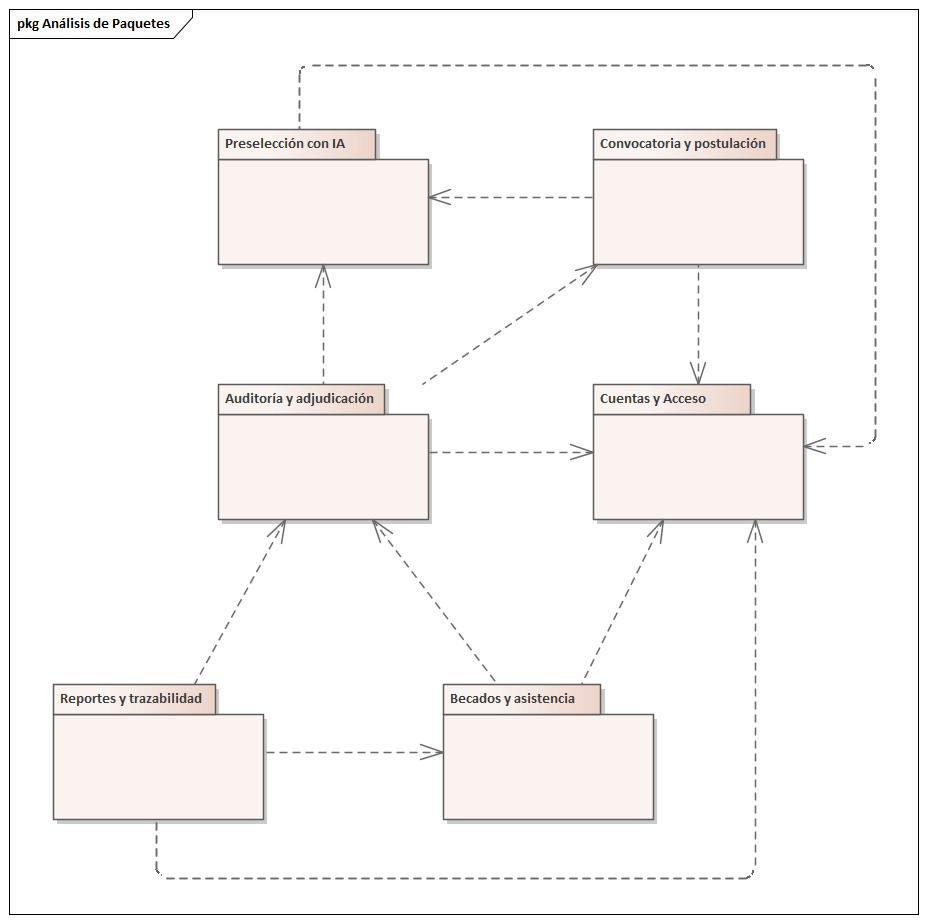
\includegraphics[width=\textwidth,height=0.85\textheight,keepaspectratio]{images/028_Analisis_Paquetes.jpg}

\smallskip
\noindent\raggedright\textit{Nota.} Elaboración propia.
\end{figure}
